\documentclass[12pt]{article}
\usepackage{tikz}
\usetikzlibrary{calc}
\usepackage{amsmath,amsthm,amssymb}
\usepackage{tikz}
\usepackage[utf8]{inputenc}
\usepackage{color}

\begin{document}

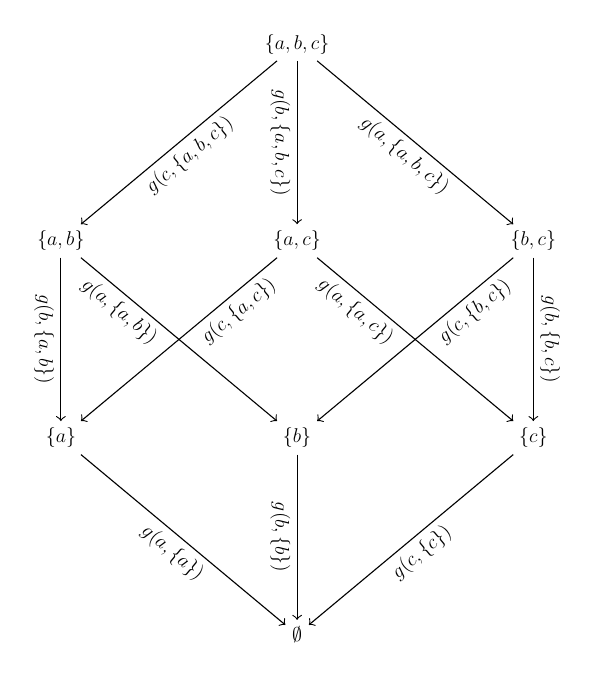
\begin{tikzpicture}[scale=.5, transform shape]
    \Large
    \tikzstyle{every node} = [rectangle]
    
    %level 0
        \node (a) at (6,0) {$\emptyset$};
        
    %level 1
        \node (b) at (0,5) {$\{a\}$};
        \node (c) at (6,5) {$\{b\}$};
        \node (d) at (12,5) {$\{c\}$};
        
    %level 2
        \node (e) at (0,10) {$\{a,b\} $};
        \node (f) at (6,10) {$\{a,c\}$};
        \node (g) at (12,10) {$\{b,c\}$};

    %level 3
        \node (h) at (6,15) {$\{a,b,c\}$};
        
    %edges
        \draw [->] (h) -- (f) node[midway, below, sloped] {$g(b,\{a,b,c\})$};
        \draw [->] (h) -- (g) node[midway, below, sloped] {$g(a,\{a,b,c\})$};  
        \draw [->] (h) -- (e) node[midway, below, sloped] {$g(c,\{a,b,c\})$}; 

        
        \draw [->] (e) -- (b) node[midway, below, sloped] {$g(b,\{a,b\})$}; 
        \draw [->] (e) -- (c) node[pos=.25, below, sloped] {$g(a,\{a,b\})$};
        \draw [->] (f) -- (b) node[pos=.25, below, sloped] {$g(c,\{a,c\})$};
        \draw [->] (f) -- (d) node[pos=.25, below, sloped] {$g(a,\{a,c\})$};
        \draw [->] (g) -- (c) node[pos=.25, below, sloped] {$g(c,\{b,c\})$};
        \draw [->] (g) -- (d) node[midway, above, sloped] {$g(b,\{b,c\})$}; 

        \draw [->] (b) -- (a) node[midway, below, sloped] {$g(a,\{a\})$};
        \draw [->] (c) -- (a) node[midway, below, sloped] {$g(b,\{b\})$};
        \draw [->] (d) -- (a) node[midway, below, sloped] {$g(c,\{c\})$};
    
    \end{tikzpicture}

\end{document}